\documentclass[12pt, letterpaper]{article}
\usepackage[utf8]{inputenc}
\usepackage[margin=1in]{geometry}
\usepackage{siunitx}
\usepackage{siunitx}
\sisetup{output-exponent-marker=\ensuremath{\mathrm{e}}}

\usepackage{float}
\usepackage[labelfont=bf, skip=5pt, font=small]{caption}
\usepackage[font={sf,small,it}]{caption}
\usepackage{natbib}
\usepackage{cite}
\usepackage{textcomp}
\usepackage{pgfplots, pgfplotstable}
\usepackage{listings}
\usepackage{verbatim}
\usepackage{alltt}
\usepackage{subfig}
\usepackage{xurl}
\usepackage{hyperref}
\usepackage{enumitem}

\usepackage{minted}
\usepackage{xcolor} % to access the named colour LightGray
\definecolor{LightGray}{gray}{0.9}
\usepackage{physics}
\usepackage{amsfonts, amsmath, amsthm, amssymb, bm}
\usepackage{blindtext}
\usepackage{enumitem}

\usepackage{array}
\newcolumntype{P}[1]{>{\centering\arraybackslash}p{#1}}
\newcolumntype{M}[1]{>{\centering\arraybackslash}m{#1}}
\usepackage{graphicx}

\usepackage{thmtools}
\usepackage[T1]{fontenc}

\newenvironment{algorithm}
 [1]
 [Default value of  argument if none provided]
{\refstepcounter{algorithm}
\fontfamily{cmss} \selectfont 
}
{
\vspace{\baselineskip}
\noindent             
 }

\usepackage{comment}

\setlength{\parskip}{1em}
\setlength{\parindent}{0em}

\usepackage{xcolor}
\definecolor{atomictangerine}{HTML}{F79256}
\definecolor{bluesapphire}{HTML}{326273}

\usepackage{hyperref}
\hypersetup{
    colorlinks=true,
    linkcolor=bluesapphire,
    filecolor=magenta,      
    urlcolor=atomictangerine,
    citecolor=bluesapphire,
    pdftitle={Overleaf Example},
    pdfpagemode=FullScreen,
    }


\begin{document}



\begin{titlepage}
   \begin{center}
       \vspace*{1cm}

       \textbf{Factor Analysis on Chemical Abundance Spaces}

       \vspace{0.5cm}
        Summer 2022 ASC \\
        u7281660
       \vspace{1.5cm}
       \textbf{Yangda Bei \\
       1$^{\text{st}}$ year}
       \vfill
       \vspace{0.8cm}
   \end{center}
\end{titlepage}

\begin{abstract}
    Factor Analysis is a statistical machine learning model used to describe the variability of correlated variables that are observed, identifies a structure that underlies them, and transforms their correlation into underlying latent factors. 
    Using Factor Analysis to approach the problem of reducing the dimensionality of stellar chemical space could provide a better understanding of how stars come into formation than Principal Component Analysis. We create an exploratory factor analysis model using a maximum likelihood SVD-based approach in Python. Applying this model to the high-dimensionality stellar chemical space of the GALactic Archaeology with Hermes survey for future work is a promising step towards providing evidence for the estimated number of dimensions of the space defined by the stellar chemical element abundances.
\end{abstract}

\pagebreak

\tableofcontents

\pagebreak

\section{Introduction}

Observational study of individual stars paired with probabilistic models provides detailed insight into the evolutionary history of galaxies. To reconstruct the order of events involved in the formation of the galactic disk of the Milky Way, the re-assembly of star-forming aggregates is crucial.


Many large-scale surveys of the Milky Way have allowed the tracing of stars through the galaxy's evolution to become increasingly possible
(e.g. RAVE - \citeauthor{rave2006} \citeyear{rave2006}; LAMOST - \citeauthor{zhao2012lamost} \citeyear{zhao2012lamost}; GALAH - \citeauthor{desilva2015} \citeyear{desilva2015}; \emph{Gaia} - \citeauthor{refId0} \citeyear{refId0}; APOGEE - \citeauthor{majewski2017} \citeyear{majewski2017}). However, due to disruptions of a star's path through the galaxy, e.g. by mass loss due to stellar evolution or gravitational interactions throughout its life, kinematic information alone is not reliable in extracting information. Although individual clusters formed from stars are chemically homogeneous (De Silva et al. \citeyear{desilva2006,desilva2007}; \citeauthor{bovy2016} \citeyear{bovy2016}), most clusters dissipate and evolve dynamically resulting in the loss of dynamical information. However, the surface chemical composition of stars provides critical insight into their history as stars that have dispersed but were born in the same cluster will have similar chemical abundance patterns, therefore, reflecting their origin and chemical evolution of the gas from which they formed.


The stellar chemical space ($\mathcal{C}$-space) is the space of measurable abundances of chemical elements. We can employ a technique named chemical tagging, a process that groups stars based on their positions in the chemical space \citep{freeman2002}, to attempt to reconstruct ancient star-forming aggregates involved in the formation of the Galactic disk. Successful chemical tagging to recover the dispersed aggregates requires precise spectroscopic data from a large number of stars. 

Before applying chemical tagging to a spectral dataset obtained from the GALactic Archaeology with HERMES (GALAH) survey, we first apply our model on a mock data sample. We aim to mimic GALAH's measurement of a 25-dimensional chemical abundance space. However, because many parts of a star's spectra rely on the same element and will therefore be correlated due to underlying nucleosynthetic processes, it is estimated that around seven chemicals are independent and that the production of others strongly correlates with them. Ting et al. (\citeyear{ting2012}) performed PCA analysis on [X/Fe] space to estimate the dimensionality of the $\mathcal{C}$-space available to HERMES, and found that the 17 elements measured can be represented in six dimensions both at high and low metallicity. It is estimated that the full 25-element HERMES space would give about eight or nine dimensions for the HERMES chemical space.


The bulk of this report will introduce factor analysis (FA), the model that aims to determine the driving factors of nucleosynthetic processes, how it differs from principal component analysis (PCA), and a comparison of our own factor model on a mock data sample against the \texttt{FactorAnalyzer} package created by \texttt{scikit-learn}.


This study served as an introduction to unsupervised machine learning algorithms, applying data analysis using Python, and placing the model into the context of determining the dimensionality of $\mathcal{C}$-space.


\section{Stellar Processes}
Metallicity is the abundance of elements that is higher than hydrogen and helium on the periodic table. The abundances of the heavy elements come from stellar nucleosynthesis and are formed in the cores of stars as they evolve over time. Metals are deposited via stellar winds and supernovae which enriches the interstellar medium to form new stars. It follows that older stars have lower metallicities than younger stars which formed in a more metal-rich universe. 

The dimensionality of the $\mathcal{C}$-space is affected largely by the interplay of stellar processes. Although stars born from the same gas formations disperse, their element abundances would remain similar. The gas itself would have its own history of pollution from core-collapse supernovae, Type Ia supernovae (SNe Ia), stellar winds from asymptotic giant branch (AGB) stars, and neutron star mergers. The high dimensionality of $\mathcal{C}$-space relies on the interplay of these processes but we think that it is driven by 5-6 underlying factors which help form the chemical makeup of the space. 

Whilst core-collapse releases metals into the interstellar medium, it does not account for every element. Neutron capture processes ($n$-capture) refer to the synthesis of heavier elements at lower temperatures due to their neutral charge so it does not get repulsed by nuclei. The majority of neutrons in supernovae do not participate in nucleosynthesis as the majority are trapped in the collapsing core \citep{thompson2001physics}. $N$-capture processes are split up into two processes: the rapid ($r$-) and slow ($s$-) processes. The $r$-process produces highly unstable nuclei for the nucleosynthesis of elements heavier than zinc through the bombardment of neutrons that rapidly decays $\beta$-decays into more stable forms. Gravitational forces during neutron star/black hole or double-neutron star mergers can pull the neutron star apart, resulting in many neutron captures and ejection of processed material \citep{lattimer1977decompression}. However, neutron-star mergers are rare occurrences since two massive stars must explode as supernovae and their residuals form a sufficiently close binary system to merge within the age of the Universe \citep{abbott2017gw170817}. In supernovae, the $r$-process is responsible for around half of all isotopes of elements heavier than iron \citep{qian1998}.

Radioactive decay in the $s$-process on the other hand happens before another neutron is captured. This slow process produces nuclei close to the valley of stability which prefers almost-stable nuclei with small $n$-capture reaction rates as the neutron flux is not so intense. The production sites of the main component of the $s$-process that produces heavy elements beyond Sr and Y are believed to mainly in low-mass asymptotic giant branch stars \citep{boothroyd2006heavy}.

Stellar winds are flows of gas ejected from the upper atmosphere of a star. Post-main-sequence stars lose nearing the end of their lifetime eject large amounts of mass, about $10^{-3}$ solar masses per year \citep{mattson2011}. For larger stars, shedding as much as 50\% of its mass clearly has a significant impact on its later stages of evolution. Intermediate mass stars become white dwarfs rather than exploding as supernovae if enough mass has been lost in their stellar winds. 

SNe Ia is the last nucleosynthesis event to contribute to the composition of the Galaxy. They require first the evolution into white dwarfs in a close binary system, followed by either spiraling together or mass transfer through the release of gravitational waves. If they can combine, once past the ``critical mass'', they reignite and trigger a supernova explosion in some cases to produce nuclei from silicon to iron peak. Its entire mass is ejected into the surrounding Galaxy and enriches the interstellar medium. We get that $\alpha$-elements, such as O, Ne, Mg, Si, S and Ca are mainly produced by core-collapsing supernovae whereas SNe Ia produces iron peak elements, such as Cr, Mn, Ni and Fe.

These nucleosynthetic processes underpin the motivation for searching for the driving elements as we can then trace the formation of star aggregates. In the following sections, we introduce the model that will allow us to find the underlying factors. Interpreting the factors of real spectral data is left for future work.




\section{PCA vs. FA}

    \subsection{Principal Component Analysis}
    
    PCA is a machine learning technique used to reduce the dimension of a data-set. Most of the time, we cannot expect the training data to densely populate the space for high-dimensional problems, and so, whilst the data vectors may have a large dimension, they will typically lie close to a much lower dimensional ``manifold'', meaning that the distribution of the data is constrained heavily \citep{barber_2018}. 
    
    From Chapter 15.2: \emph{Principal Component Analysis} \citep{barber_2018}, a datapoint $\vb{x}^n$ can be approximated to a lower dimensional coordinate system as 
    $$\vb{x}^n \approx \vb{c}+\sum^{M}_{j=1}y^n_j\vb{b}^j \equiv \Tilde{\vb{x}}^n,$$
    where $\vb{b}^j$ are the ``basis'' vectors that span the linear subspace that is fitted to the data (or ``principal component coefficients'') and $y^n_i$ are the low dimensional coordinates of the data which forms a lower dimension $\vb{y}^n$ for each datapoint $n$ for components $i=1,\dots,M$. The optimal bias $\vb{c}$ is given to be the mean of the data and centres the coordinate system of the linear subspace.
    
    To find the components, one way is to use \emph{Singular Value Decomposition} (SVD) on a matrix $\vb{X}\in\mathbb{R}^{D\times N}$, given by
    $$\vb{X = UDV}^T,$$
    where $\vb{U}\in\mathbb{R}^{D\times D}$ satisfying $\vb{U}^T \vb{U} = \vb{I}$, $\vb{V}\in\mathbb{R}^{N\times N}$ satisfying $\vb{V}^T \vb{V} = \vb{I}$, and $\vb{D}$ is a $D\times N$ diagonal matrix of the positive singular values. $\vb{D}$ is assumed to have its singular values ordered with the upper left diagonal element to be the largest and so we can write the matrix $\vb{XX}^T$ as
    $$\vb{XX}^T = \vb{UDV}^T\vb{VD}^T\vb{U}^T = \vb{U}\Tilde{\vb{D}}\vb{U}^T,$$
    where $\Tilde{\vb{D}}\equiv\vb{DD}^T$ is a $D\times D$ diagonal matrix with $N$ squared singular values on the main diagonal. We can see that $\vb{U}\Tilde{\vb{D}}\vb{U}^T$ is in the form of an eigen-decomposition and so the solution is the same as the SVD decomposition of $\mathbf{X}$.
    
    PCA components are orthogonal linear combinations that maximise total variance. However, interpreting the actual components is not so straightforward. PCA has been used to reduce the dimensionality of the $\mathcal{C}$-space and the respective components were used to interpret stellar chemistry evolution processes as explored by Ting et al. (\citeyear{ting2012}) (PCA) and Price-Jones \& Bovy (\citeyear{bovy2017}) (expectation maximised PCA).
    
    Now, we present an alternative component recovery method to PCA: FA, a method that searches for hidden ``factors'' to explain the correlation between observed variables.
    
    \subsection{Factor Analysis}
    
    FA is a latent linear model that searches for influential underlying factors (or the latent variables) from a set of observed variables. FA fundamentally differs from PCA in the way that it approaches the problem of approximation to a low dimensional manifold. Instead of  optimally creating components that form a larger set of variables through linear combinations, FA instead aims to express each variable as a weighted combination (factor loadings) of hypothesised latent factors with some added noise.

    There are two types of factor models generally accepted (\citeauthor{decoster1998overview} \citeyear{decoster1998overview}, \citeauthor{kline2014easy} \citeyear{kline2014easy}): exploratory factor analysis and confirmatory factor analysis. The main difference between the two is exploratory factor analysis aims to discover the nature of constructs influencing observed variables and confirmatory factor analysis have \emph{a priori} assumptions made about the underlying constructs and sets to test whether they behave in a predicted way.

    
    From Chapter 21.1: \emph{Factor Analysis} \citep{barber_2018}, our factor model aims to find a lower dimensional probabilistic description of a dataset given by
    $$\vb{V} = \{\vb{v}^1,\dots,\vb{v}^N\}$$
    where $\dim{(\vb{v})}=D$.
    
    If our dataset lies close to a $H$-dimensional linear subspace, we can project each datapoint to the subspace and accurately approximate them using the $H$-dimensional coordinate system, similar to PCA.
    
    We attempt to explain a set of $D$ observations in each of $N$ individuals in $\vb{V}$ with a set of $H$ common factors where there are fewer factors than observations ($H<D$).
    
    The factor model will generate an observation based on the equation
    $$\vb{V}-\vb{M}=\vb{Fh}+\bm{\varepsilon},$$
    where $\vb{F} \in \mathbb{R}^{D\times H}$ is the factor matrix, $\vb{h}\in \mathbb{R}^{H\times N}$ is the \emph{factor loading} matrix which contains the ``weight'' of each factor, and $\bm{\varepsilon}$ is the unobserved stochastic error with zero mean and covariance $\vb{\Psi}$. $\vb{M}\in\mathbb{R}^{D\times N}$ is the mean matrix that sets the origin of the coordinate system, where $\vb{m}^i=\vb{\Bar{v}}^i$. We then set $\vb{X}\equiv \vb{V}-\vb{M}$.
    



    Figure \ref{fig:pca_vs_fa} shows graphically how the direction of influence of the two techniques are reversed. We see that FA assumes that observable variables are based on underlying factors whereas components are defined as measured responses. Exploratory FA also assumes that the variance in the measured variables can be decomposed into that accounted for by common factors and that accounted for by unique factors. The principal components are defined simply as linear combinations of the measurements, and so will contain both common and unique variance.


    The choice of covariance also differs between PCA and FA. Both methods aim to provide a ``low-rank'' (limited number of principal components or latent factors used) approximation from a given covariance (or correlation) matrix. For a $D\times D$ covariance matrix $\vb{\Sigma}$, we have that 
    \begin{align*}
        \text{PCA} &: \vb{\Sigma}\equiv \vb{WW}^T \\
        \text{PPCA} &: \vb{\Sigma}\equiv \vb{WW}^T + \sigma^2\vb{I} \\
        \text{FA} &: \vb{\Sigma}\equiv \vb{FF}^T+\vb{\Psi}
    \end{align*}
    where $\vb{\Psi}=\text{diag}(\psi_1,\dots,\psi_D)$ and $\vb{W}\in\mathbb{R}^{D\times H}$ is the matrix representing $H$ principal components. PPCA stands for \emph{probabilistic PCA} which is an intermediate model complexity between PCA and FA. It takes the $H$ principal eigenvalues and their corresponding eigenvectors of the sample covariance matrix. This serves as a useful initialisation for FA.
    
    We see that FA differs from PCA through $\text{diag}(\vb{\Sigma})$. As the dimensionality $D$ increases, the diagonal has a lesser impact since there are only $D$ elements on the diagonal and $D(D-1)/2 = \mathcal{O}(D^2)$ elements off the diagonal. Therefore, FA models the ``common part'' of the matrix by taking into account all the off-diagonal elements and the common part of the diagonal, providing a richer description of the off-subspace noise $\vb{\Psi}$. PCA therefore explains variance but explains correlations imprecisely for a smaller number of observed dimensions. FA explains correlations but cannot account (using the common factors) as much data variation as PCA can.
    
    
    \begin{figure}
        \centering
        \subfloat[\centering Factor model]{{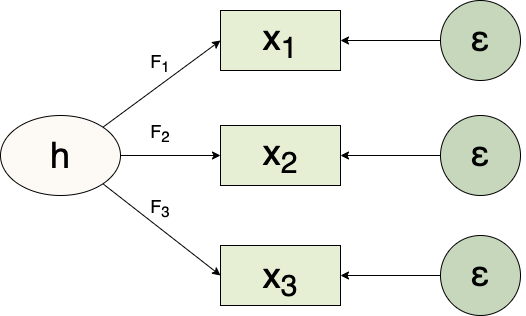
\includegraphics[width=7.5cm]{fa.drawio.png} }}%
        \quad\quad\quad\quad\quad
        \subfloat[\centering Component model]{{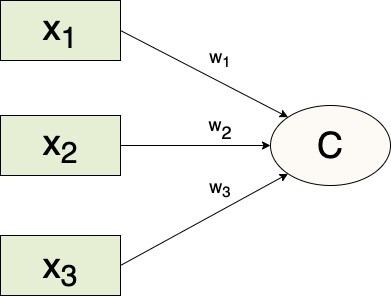
\includegraphics[width=5.8cm]{pca.drawio.png} }}%
        \caption{Factors are latent variables that explain the covariances (correlations) between observed variables. Components are a linear summation of variables and do not necessarily reveal the correlations between them. The correlations between the variables in the factor equation are expressed in terms of the factor loadings ($\mathbf{\mathbf{h}}$) which is then multiplied by the factors ($\mathit{\mathbf{F}_i}$) to give the observed variables ($\mathbf{x}_i$). Noise ($\mathbf{\varepsilon}$) is then added to give the final variable. The component equation shows components ($\mathit{\mathbf{C}}$) represented as a linear combination of the variables ($\mathit{\mathbf{x}_i}$) and their weights ($\mathit{w_i}$). Observed variables are represented by boxes and unobserved components are represented in ellipses. Graphs created using \href{http://draw.io}{\emph{\texttt{draw.io}}}}%
        \label{fig:pca_vs_fa}
    \end{figure}

\section{Implementation}

We attempt to build from scratch an FA model as an exercise in data analysis and modelling in Python. The \texttt{FactorAnalyzer} package created by \texttt{scikit-learn} was used as a benchmark to compare the recovery of the mock latent factors. \texttt{FactorAnalyzer} performs a maximum likelihood estimate of the factor loading matrix using an SVD-based approach \citep{scikit-learn} \footnote{\url{https://github.com/scikit-learn/scikit-learn/blob/main/sklearn/decomposition/_factor_analysis.py}}. Our rudimentary model uses the same method following Algorithm 21.1 \citep{barber_2018}.

The companion Jupyter Notebook to the report can be found at \url{https://github.com/yangdabei/factor-analysis}. 

\pagebreak

\textbf{Algorithm 21.1}
\begin{algorithm}[21.1]
    \vspace{-10px}

    \begin{enumerate}[nosep,nolistsep]
    
    \item
    Initialise the diagonal noise $\vb{\Psi}$.
    
    \item
    Find the mean $\vb{\Bar{v}}$ of the data $\vb{v}^1,\dots,\vb{v}^N$.
    
    \item
    Find the variance $\sigma_i^2$ for each component $i$ of the data $v_i^1,\dots,v_i^N$.
    
    \item
    Compute the centred matrix $\vb{X}=[\vb{v}^1-\vb{\Bar{v}},\dots,\vb{\Bar{v}}^N-\vb{\Bar{v}}]$
    
    \item
    \verb|while| Likelihood not converged or termination criterion \verb|not| reached \verb|do|
    \end{enumerate}
    
    \begin{enumerate}[resume,nosep,nolistsep, leftmargin=2.2cm]
    \vspace{-11px}
    \item 
    Form the scaled data matrix $\vb{\Tilde{X}}=\vb{\Psi}^{-\frac{1}{2}}\vb{X}/\sqrt{N}$.
    
    \item 
    Perform SVD for $\vb{\Tilde{X}}=\vb{U\Tilde{\Lambda}\Tilde{W}^T}$ and set $\vb{\Lambda}=\vb{\Tilde{\Lambda}}^2$
    
    \item 
    Set $\vb{U}_H$ to the first $H$ columns of $\vb{U}$ and set $\vb{\Lambda}_H$ to contain the first $H$ diagonal entries of $\vb{\Lambda}$.
    
    \item 
    $\vb{F}=\vb{\Psi}^{\frac{1}{2}}\vb{U}_H(\vb{\Lambda}_H-\vb{I}_H)^{\frac{1}{2}}$
    \hfill
    $\triangleright \quad$ \hspace{0.23cm}\texttt{factor update}
    
    \item 
    $L=\frac{N}{2} \left\{ \sum^H_{i=1}\log\lambda_i +H +\sum^D_{i=H+1}\lambda_i + \log\det(2\pi\Psi)\right\}$
    \hfill
    $\triangleright \quad$ \texttt{log likelihood}
    
    \item 
    $\vb{\Psi} = \text{diag} \left(\vb{\sigma}^2\right) - \text{diag}\left(\vb{FF^T}\right)$
    \hfill
    $\triangleright \quad\quad$ \texttt{noise update}
    \end{enumerate}
    
    \begin{enumerate}[resume, nosep, topsep=0pt]
    \vspace{-11px}
    \item
    \verb|end while|
    
    \end{enumerate}

\end{algorithm}

First we set some initial constants:
\begin{minted}[
frame=lines,
framesep=2mm,
baselinestretch=1.2,
bgcolor=LightGray,
fontsize=\footnotesize,
linenos,
firstnumber=last
]
{python}
import numpy as np

# initial constants and variables
L_old = -np.infty
# error tolerance
tol = 1e-3 
# max iterations before termination
max_iter = 100 
\end{minted}
The following code blocks correspond to the steps of the algorithm:
\begin{minted}[
frame=lines,
framesep=2mm,
baselinestretch=1.2,
bgcolor=LightGray,
fontsize=\footnotesize,
linenos
]
{python}
# 1. Initialise diagonal noise
noise = 0.01*np.random.normal(size=(num_dimension,num_dimension))
psi = np.diag(np.diag(np.cov(noise)))
\end{minted}
\vspace{-40px}
\begin{minted}[
frame=lines,
framesep=2mm,
baselinestretch=1.2,
bgcolor=LightGray,
fontsize=\footnotesize,
linenos,
firstnumber=last
]
{python}
# 2. Find the mean of the data
result = []
for vector in V:
    result.append([sum(vector)/len(vector)])

M = np.array(result)
\end{minted}
\vspace{-40px}
\begin{minted}[
frame=lines,
framesep=2mm,
baselinestretch=1.2,
bgcolor=LightGray,
fontsize=\footnotesize,
linenos,
firstnumber=last
]
{python}
#3. Find the variance
var = np.var(V, axis=0)
\end{minted}
\vspace{-40px}
\begin{minted}[
frame=lines,
framesep=2mm,
baselinestretch=1.2,
bgcolor=LightGray,
fontsize=\footnotesize,
linenos,
firstnumber=last
]
{python}
# 4. Compute the centred matrix
X = V - M
\end{minted}
\vspace{-40px}
\begin{minted}[
frame=lines,
framesep=2mm,
baselinestretch=1.2,
bgcolor=LightGray,
fontsize=\footnotesize,
linenos,
firstnumber=last
]
{python}

# 5. While loop runs if error is greater than tolerance or until max_iter
for i in range(max_iter):
    #----------------------------------------------------------------------------
    # 6. Form the scaled data matrix
    X_tilde = np.dot(np.linalg.inv(np.sqrt(psi)), X.T / (num_sample ** 0.5))
    #----------------------------------------------------------------------------
    # 7. Perform SVD for the scaled data matrix
    U,Lambda_tilde,VT = np.linalg.svd(X_tilde)
    Lambda_tilde = np.diag(Lambda_tilde)
    Lambda = Lambda_tilde ** 2
    #----------------------------------------------------------------------------
    # 8. Set U_H to the first H columns of U and set Lambda_H to contain the 
    #    first H diagonal entries of Lambda
    H = num_latent
    U_H = U[:,:H]
    Lambda_H = Lambda_tilde[:H,:H]
    #----------------------------------------------------------------------------
    # 9. Factor update
    F = np.sqrt(psi) @ U_H @ np.sqrt(Lambda_H - np.identity(H))
    #----------------------------------------------------------------------------
    # 10. Log likelihood
    a = 0
    for j in range(H):
        a += np.log(Lambda[j,j])
    b = 0
    for k in range(H+1,num_dimension):
        b += Lambda[k,k]
    
    L_new = (num_dimension/2)*(a + H + b + np.log(np.linalg.det(2*np.pi*psi)))
    #----------------------------------------------------------------------------
    # 11. Psi update
    psi = np.maximum(np.diag(var)-np.diag(F@F.T),1e-12)
    #----------------------------------------------------------------------------
    if np.abs(L_new-L_old)<tol:
        break
    # log likelihood update
    L_old = L_new
\end{minted}

We apply the model outlined to a mock data sample and random latent factors. We first fit \texttt{FactorAnalyzer} to the mock data and call the method \texttt{.components\_} to extract the factors. Then we apply our model to the sample. The number of factors were determined prior by finding the number of eigenvalues of the correlation matrix $>1$.  \texttt{mockdata.csv} contains the mock data and \texttt{latentfactors.csv} contain the mock factors. All files can be found at \url{https://github.com/yangdabei/factor-analysis}.

Note that some true factors are used more than once to compare the package fits. This is due to how closely the $L_1$-norm fits to the true factors. To show the comparison for the factors, Figure \ref{fig:true_v_package} contrasts the true factors with the components extracted from \texttt{FactorAnalyzer} and Figure \ref{fig:true_v_model} is the difference between the true factors and our created model fit.


\section{Identifiability of Latent Factors up to a Rotation}


\begin{figure}
    \centering
    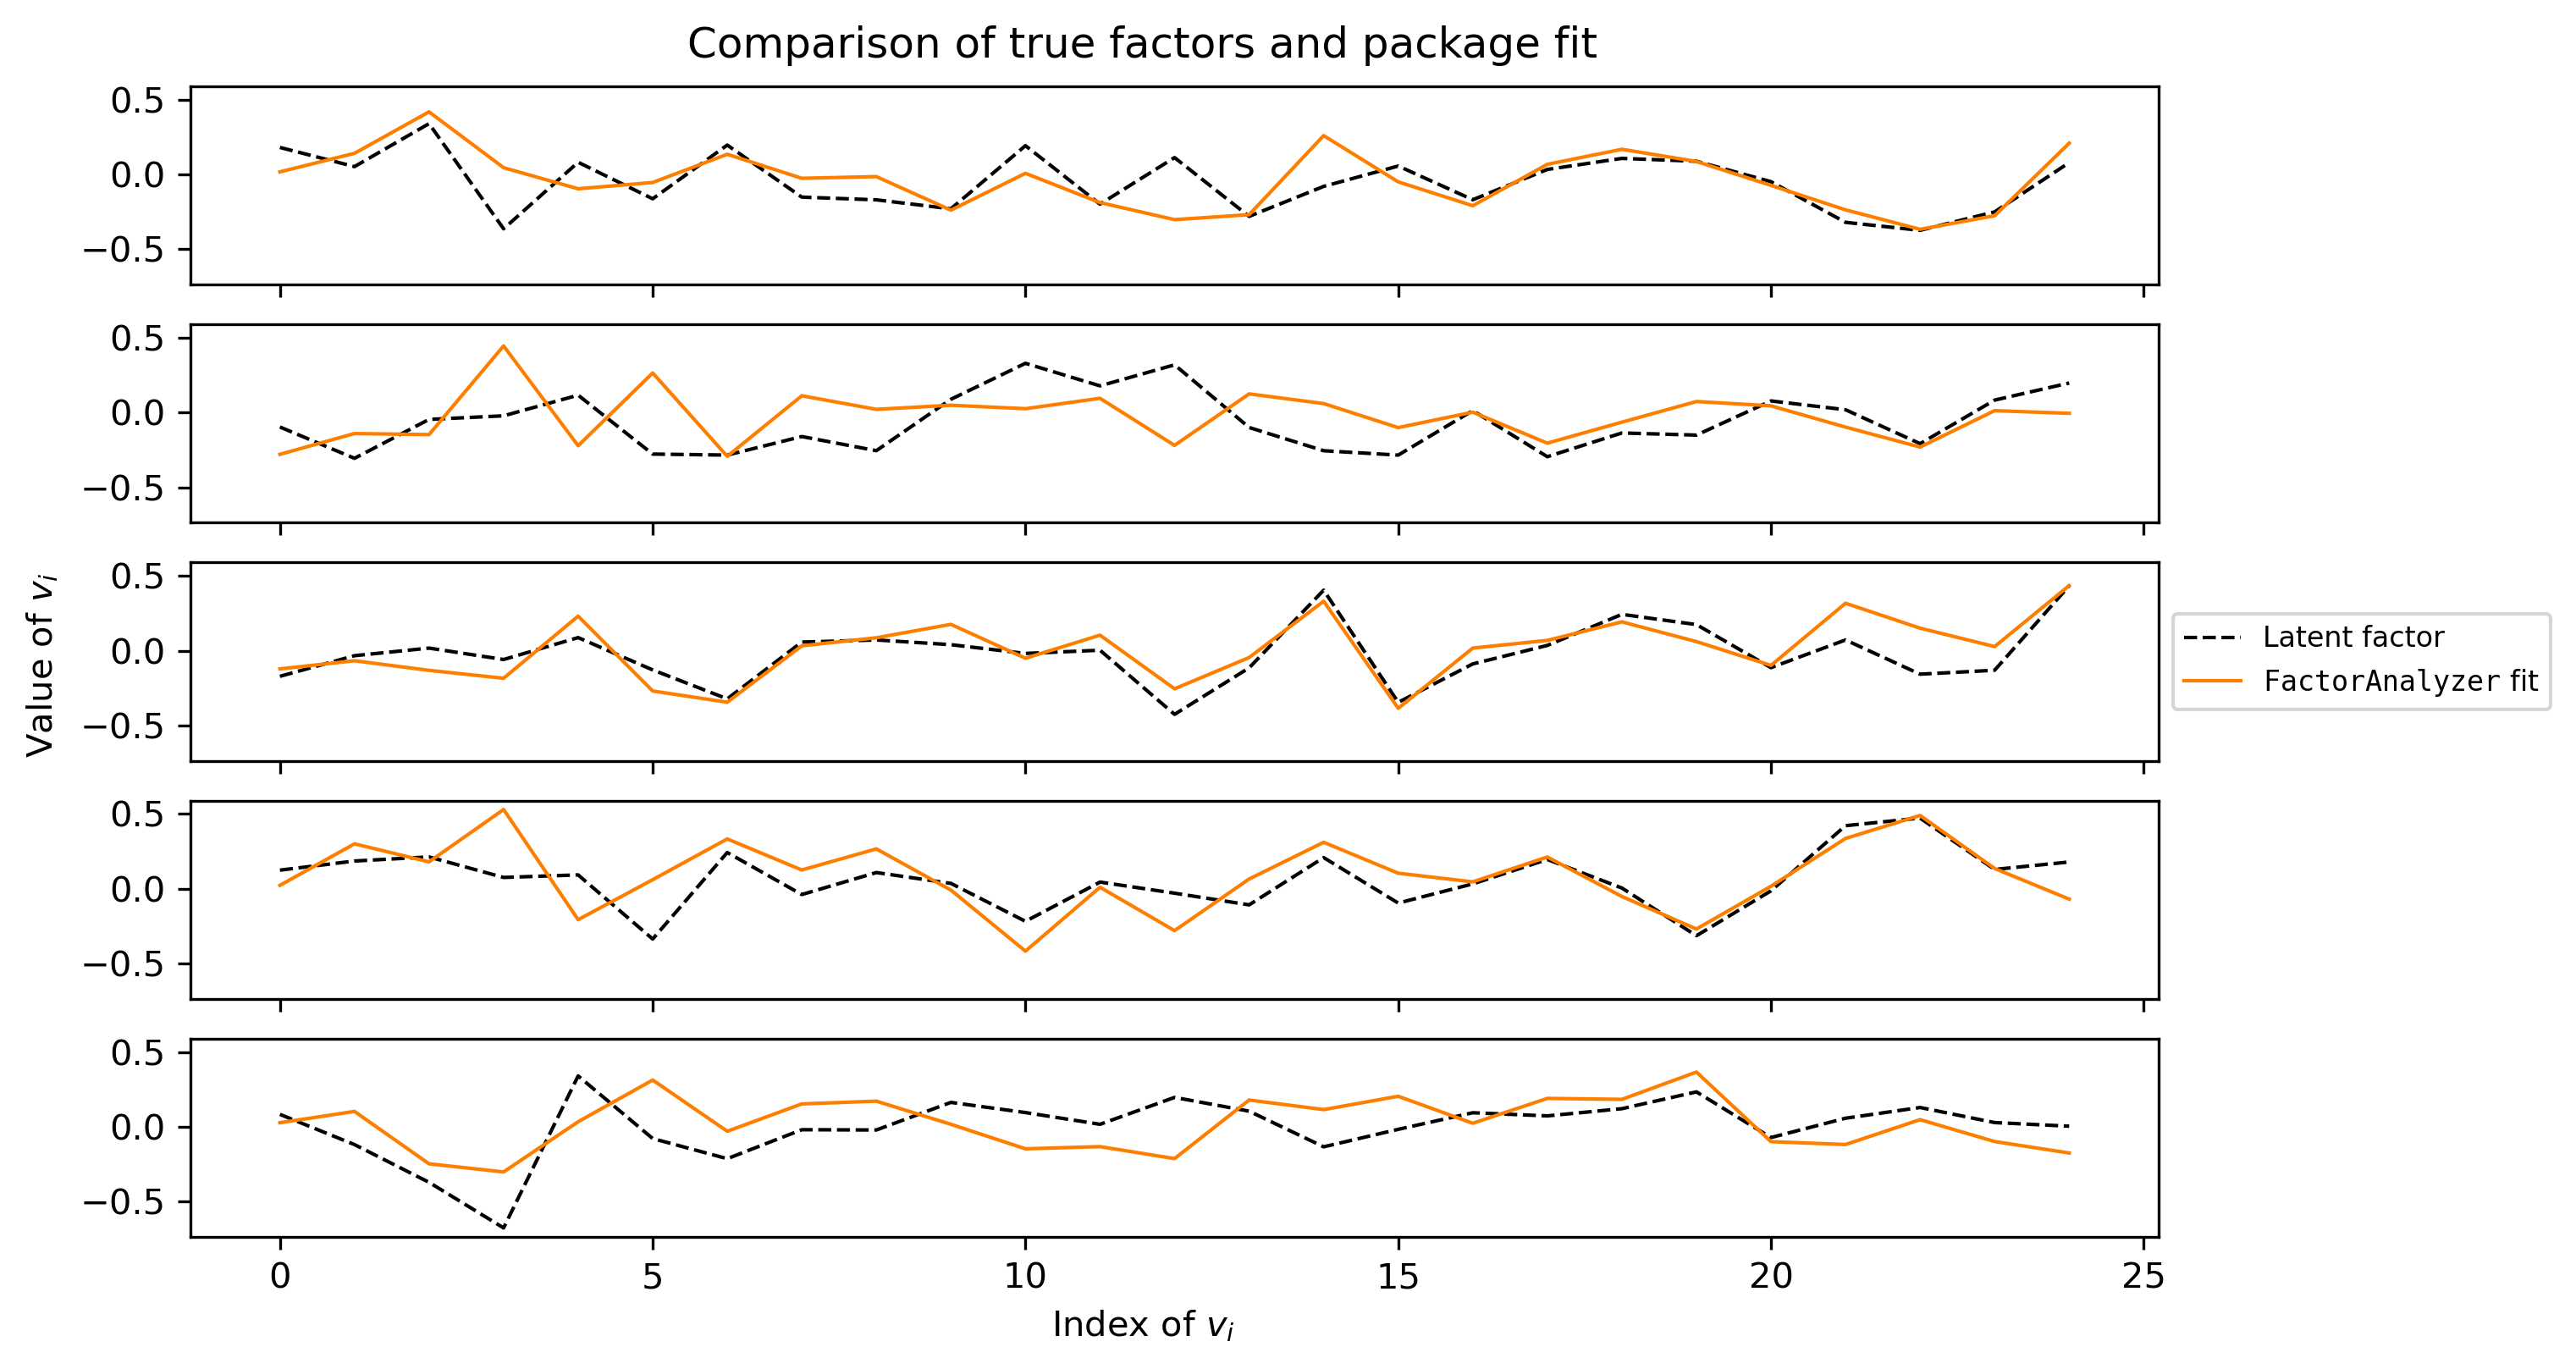
\includegraphics[width=16cm]{true_v_package.png}
    \caption{True latent factors (dashed black line) compared to the factors derived from \texttt{FactorAnalyzer} (solid orange line). }
    \label{fig:true_v_package}
\end{figure}


\begin{figure}
    \centering
    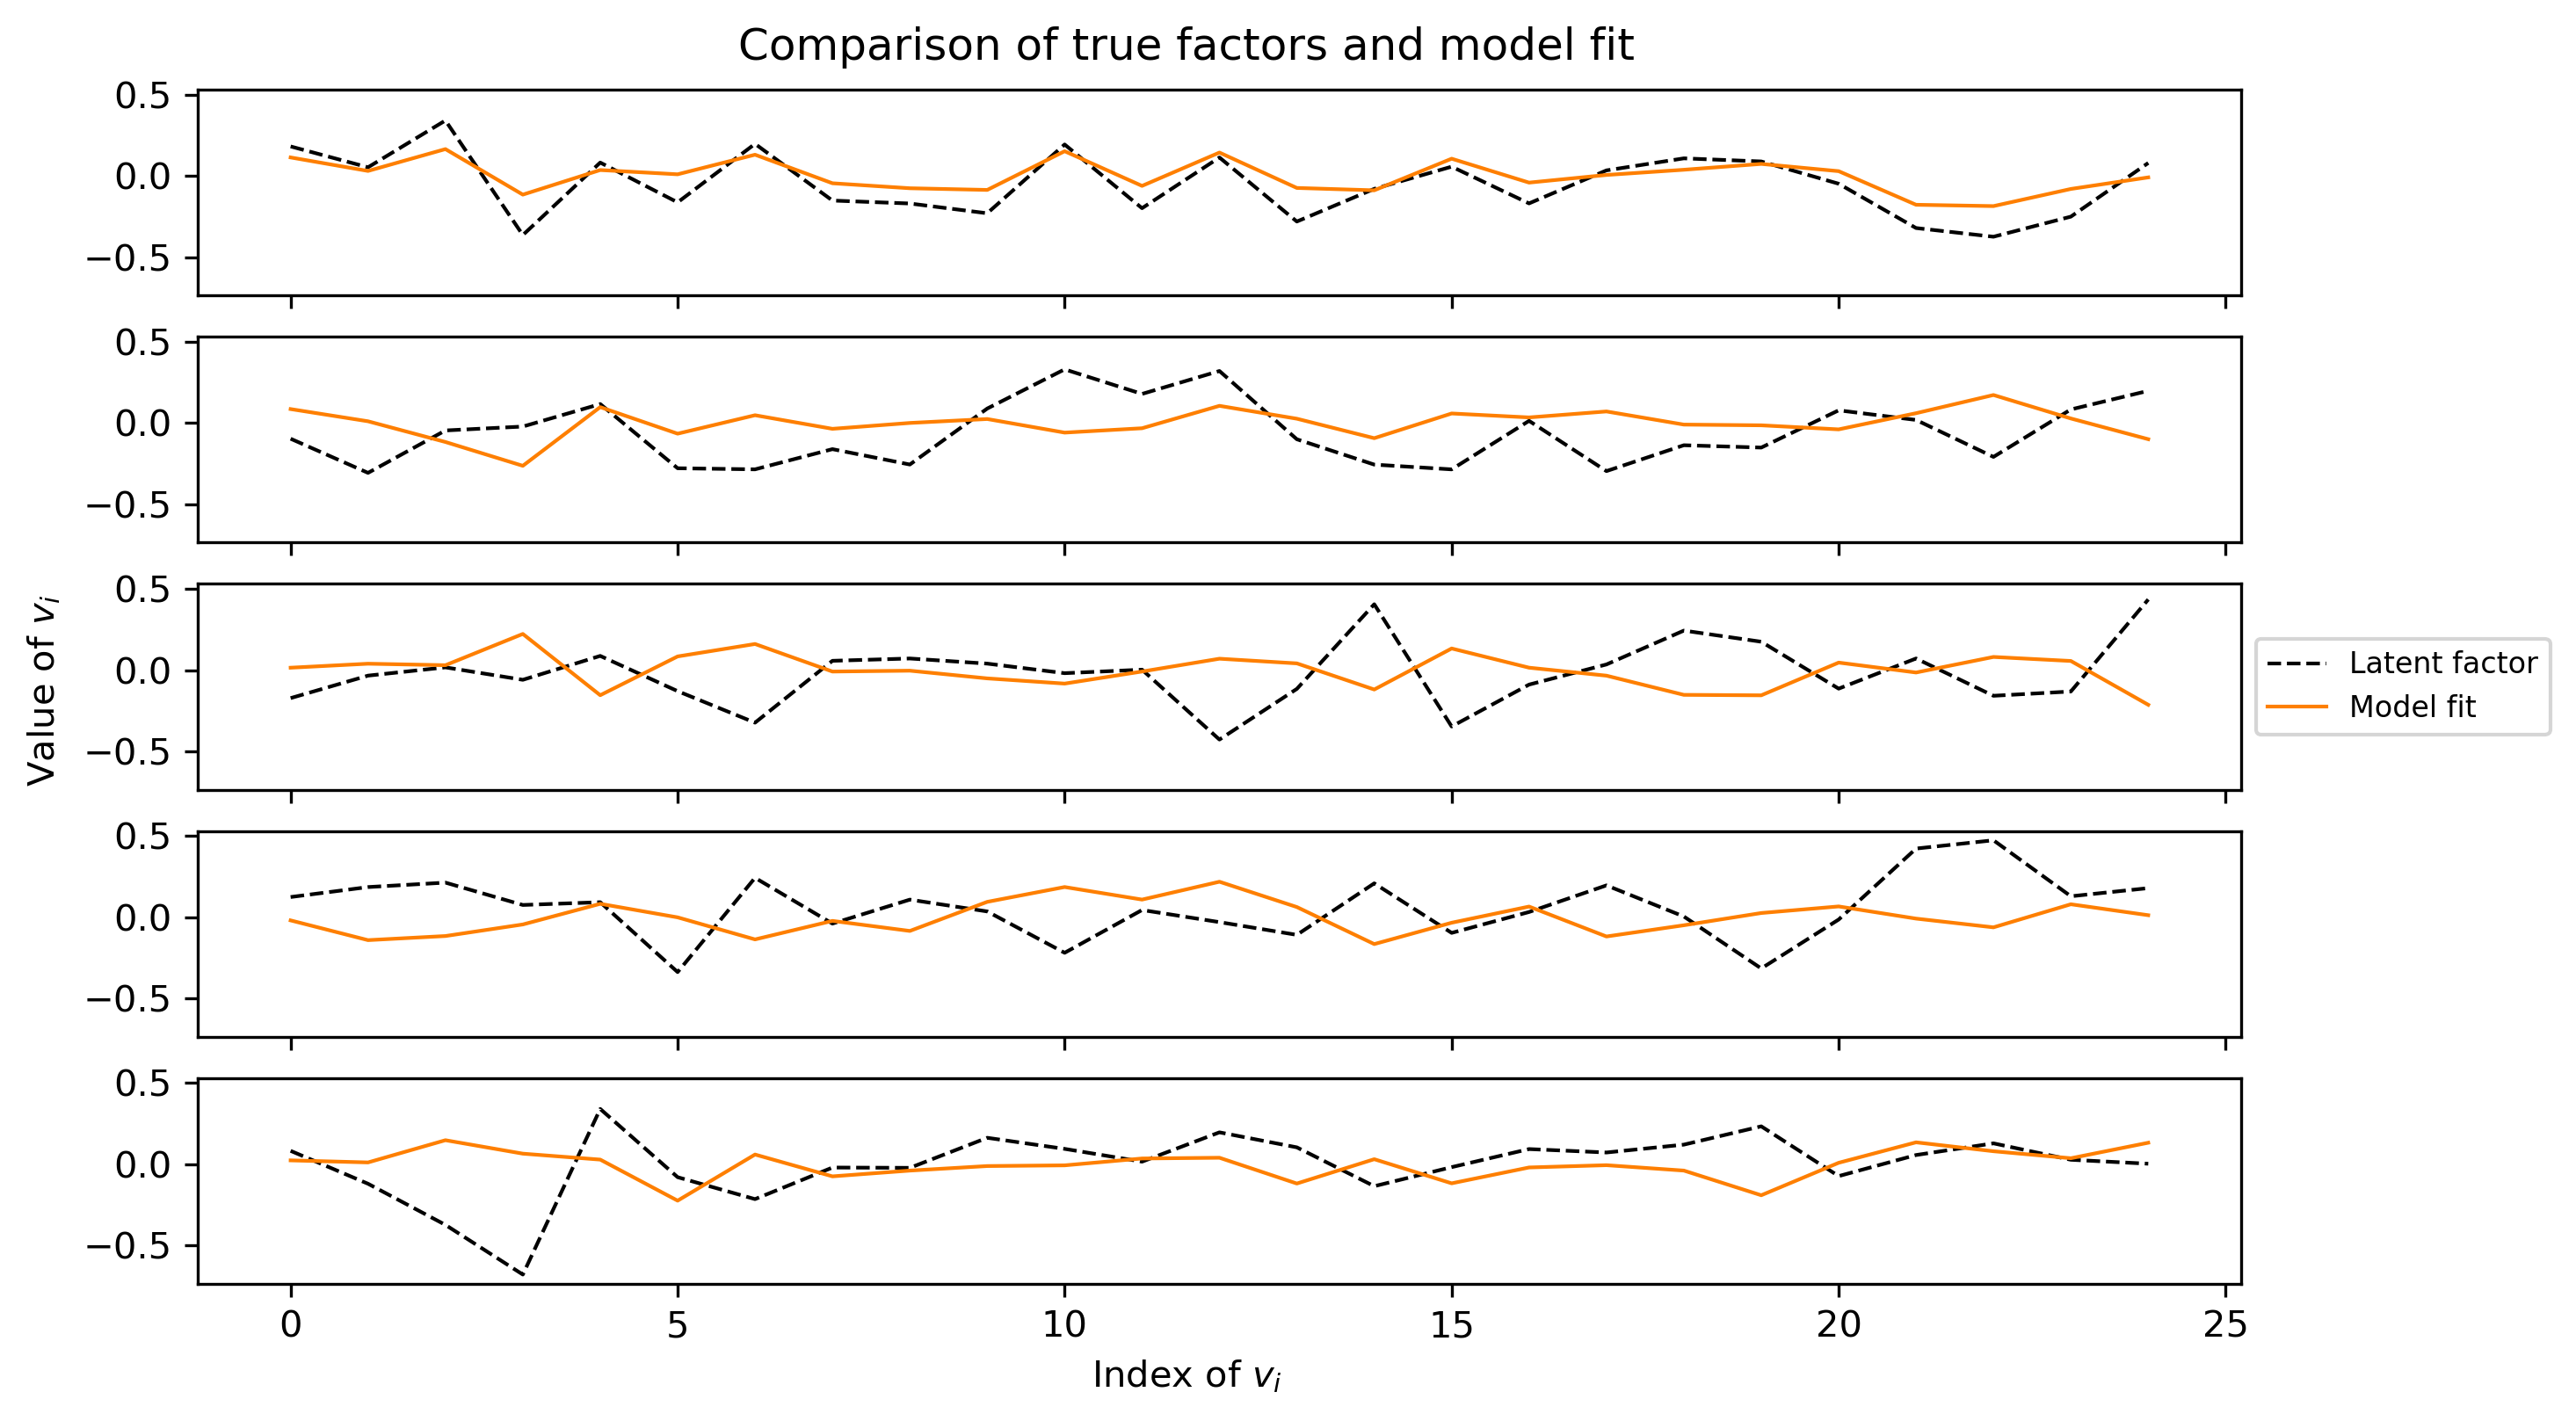
\includegraphics[width=16cm]{true_v_model.png}
    \caption{True latent factors (dashed black line) compared to the factors derived from created model (solid orange line).}
    \label{fig:true_v_model}
\end{figure}

%\begin{figure}
%    \centering
%    \includegraphics[width=16cm]{package_v_model.png}
%    \caption{\texttt{FactorAnalyzer} components and factors %derived from model.}
%    \label{fig:package_v_model}
%\end{figure}

Identifiability of factors is an issue in FA due to the nature of how the lower dimensional manifold is formed. Being able to uniquely identify the factor loading matrix and the latent factors ensures substantive interpretations to be made. Because reproduction of factors have an infinite amount of mathematically correct expressions, we need to have a way of choosing the solution which gives us the most substantive interpretations. This comes in the form of manipulating the reference axes of the spanning vectors of the subspace, also known as a rotation. 

Choosing the correct rotation can also make interpretation easier. Rotation methods are either orthogonal (assumes factors in analysis are uncorrelated) or oblique (assumes factors in analysis are correlated). \texttt{FactorAnalysis} currently has two rotation methods implemented, both of which are orthogonal: \texttt{varimax} and \texttt{quartimax}. Varimax is arguably the most popular method for orthogonal rotation where the sum of the variances of the squared loadings is maximised \citep{kaiser1958varimax}. This still preserves the orthogonality and leaves the subspace invariant.

Consider an arbitrary $H\times H$ rotation matrix $\vb{R}$, and thus satisfying $\vb{RR}^T=\vb{I}$. If we define $\Tilde{\vb{F}}= \vb{FR}^T$ and then rotate the latent factors as $\Tilde{\vb{h}}= \vb{Rh}$, we have that
$$\Tilde{\vb{F}}\Tilde{\vb{h}} = \vb{FR}^T\vb{Rh}=\vb{Fh}.$$
The covariance matrix for $\Tilde{\vb{X}}$ is 
$$\Tilde{\vb{\Sigma}}= \Tilde{\vb{F}}\Tilde{\vb{F}}^T + \vb{\Psi} = \Tilde{\vb{F}}\vb{RR}^T\Tilde{\vb{F}}^T=\vb{FF}^T+\vb{\Psi}=\vb{\Sigma}.$$
Hence, datapoints $x_i$ conditioned on latent factors $h_i$ is not identifiable due to rotational indeterminacy and can simultaneously rotate the latent factors and the factor loading matrix without changing the distribution of the data.

Since solutions are not unique and can be affected by a rotation, we want to find individual vectors that span the plane of the coordinate system. Forcing the factor matrix to be orthonormal and ordering the columns in order of decreasing variance of the corresponding latent factors means that identifiability becomes possible due to more constraints being put onto $\vb{F}$. This is ultimately the strategy that PCA adopts.

Currently, the two parameters of our model ($\mathbf{F}$, $\mathbf{\Psi}$) are not initialised, resulting in some vectors having a skewed fit in Figure \ref{fig:true_v_model}. To address the issue of rotation, if we initialise an $\mathbf{F}_0$ as the true factors with some added noise, it is expected that we can better the model. Then, whether the subspace is rotated will not play a part as the initialisation is close to the true value. At the moment of writing, the initialisation is being refined. We can initialise close to the true value for when we apply the model to spectral data.

%\subsubsection{Identifiability up to label switching}
%
%Another issue is the problem of different orderings of factors %leading. This leads to the factors being indistinguishable. Suppose %there are $H$ latent factors. If there are two different orderings of %the rows of $\mathbf{h}$ and their corresponding columns of %$\mathbf{f}$ but have an identical product, we get:
%$$\mathbf{f}_k\mathbf{h}_k = \mathbf{f}_{k'}\mathbf{h}_{k'}$$
%$$k \in {2,3,1} \quad k' \in {1,2,3}$$
%This is known as label-switching where the two orderings cannot be %distinguished based on likelihood.  





\section{Future Work}

Although we offer some comparisons in Figures \ref{fig:true_v_package} and \ref{fig:true_v_model}, it is beyond the scope of this report to interpret the factors of stellar spectra. For future observational research, we can begin to perform chemical tagging and apply our factor model to the high-resolution ($R\sim 28\,000$) stellar spectra gathered from the GALactic Archaeology with HERMES (GALAH) survey using the High Efficiency and Resolution Multi-Element Spectrograph (HERMES) instrument. From there, we can extract the latent factors of the multi-dimensional $\mathcal{C}$-space and interpret them as elements that drive stellar processes.

Further work can be done by altering the model so that it uses an ``expectation maximisation'' approach to retrieve the latent factors and to incorporate rotation methods to better fit the data.

\section{Conclusion}

The aim of this project was to be introduced to some preliminary machine learning models, FA and PCA. We created an exploratory factor model using a maximum likelihood SVD-based approach, inspired by the \texttt{FactorAnalyzer} package from the \texttt{scikit-learn} module. We then attempted to recover the latent factors from a mock data sample. There are many more features yet to be added to the model such as tackling the problem of rotations which can be solved by implementing a good initialisation $\mathbf{F}_0$ or adding a rotation optimiser. The ultimate goal is to apply the model to the spectral data gathered by the GALAH survey and to interpret the latent factors as nucleosynthetic processes.

\section{Acknowledgements}

This project was supported by Yuan-Sen Ting. Thanks is also to be given to Zechang Sun for inspiration with optimisation ideas from his factor model.

\pagebreak

\bibliographystyle{agsm}
\bibliography{references}

\end{document}